\documentclass[11pt,a4paper,oneside]{report}

% thanks to http://tex.stackexchange.com/a/47579/71109
\usepackage{pdfpages}
\usepackage{ifxetex}
\usepackage{ifluatex}
\newif\ifxetexorluatex % a new conditional starts as false
\ifnum 0\ifxetex 1\fi\ifluatex 1\fi>0
   \xetexorluatextrue
\fi

\ifxetexorluatex
  \usepackage{fontspec}
\else
  \usepackage[T1]{fontenc}
  \usepackage[utf8]{inputenc}
  \usepackage[lighttt]{lmodern}
  \ttfamily\DeclareFontShape{T1}{lmtt}{m}{it}{<->sub*lmtt/m/sl}{}
\fi

\usepackage[english,magyar]{babel} % Alapértelmezés szerint utoljára definiált nyelv lesz aktív, de később külön beállítjuk az aktív nyelvet.

\usepackage{emptypage} % omit page number on empty pages

%\usepackage{cmap}
\usepackage{amsfonts,amsmath,amssymb} % Mathematical symbols.
%\usepackage[ruled,boxed,resetcount,linesnumbered]{algorithm2e} % For pseudocodes. % beware: this is not compatible with LuaLaTeX, see http://tex.stackexchange.com/questions/34814/lualatex-and-algorithm2e
\usepackage{booktabs} % For publication quality tables for LaTeX
\usepackage{graphicx}

%\usepackage{fancyhdr}
%\usepackage{lastpage}

\usepackage{anysize}
%\usepackage{sectsty}
\usepackage{setspace} % For setting line spacing

\usepackage[unicode]{hyperref} % For hyperlinks in the generated document.
\usepackage{xcolor}
\usepackage{listings} % For source code snippets.

\usepackage[amsmath,thmmarks]{ntheorem} % Theorem-like environments.

\usepackage[hang]{caption}

\singlespacing

\newcommand{\selecthungarian}{
	\selectlanguage{magyar}
	\setlength{\parindent}{2em}
	\setlength{\parskip}{0.5em}
	\frenchspacing
}

\newcommand{\selectenglish}{
	\selectlanguage{english}
	\setlength{\parindent}{0em}
	\setlength{\parskip}{0.5em}
	\nonfrenchspacing
	\renewcommand{\figureautorefname}{Figure}
	\renewcommand{\tableautorefname}{Table}
	\renewcommand{\partautorefname}{Part}
	\renewcommand{\chapterautorefname}{Chapter}
	\renewcommand{\sectionautorefname}{Section}
	\renewcommand{\subsectionautorefname}{Section}
	\renewcommand{\subsubsectionautorefname}{Section}
}

\usepackage[numbers]{natbib}
\usepackage{xspace}


\newcommand{\vikszerzoVezeteknev}{Fintha}
\newcommand{\vikszerzoKeresztnev}{Dénes Flórián}

\newcommand{\vikkonzulensAMegszolitas}{Dr.~}
\newcommand{\vikkonzulensAVezeteknev}{Bergmann}
\newcommand{\vikkonzulensAKeresztnev}{Gábor}

\newcommand{\vikkonzulensBMegszolitas}{}
\newcommand{\vikkonzulensBVezeteknev}{}
\newcommand{\vikkonzulensBKeresztnev}{}

\newcommand{\vikkonzulensCMegszolitas}{}
\newcommand{\vikkonzulensCVezeteknev}{}
\newcommand{\vikkonzulensCKeresztnev}{}

\newcommand{\vikcim}{Performance analysis of a language tooling}
\newcommand{\viktanszek}{\bmemit}
\newcommand{\vikdoktipus}{\bsc}
\newcommand{\vikmunkatipusat}{szakdolgozatot}

\input{include/tdk-variables}
\newcommand{\szerzoMeta}{\vikszerzoVezeteknev{} \vikszerzoKeresztnev}
\input{include/thesis-en}
%--------------------------------------------------------------------------------------
% Page layout setup
%--------------------------------------------------------------------------------------
% we need to redefine the pagestyle plain
% another possibility is to use the body of this command without \fancypagestyle
% and use \pagestyle{fancy} but in that case the special pages
% (like the ToC, the References, and the Chapter pages)remain in plane style

\pagestyle{plain}
\marginsize{35mm}{25mm}{15mm}{15mm}

\setcounter{tocdepth}{3}
%\sectionfont{\large\upshape\bfseries}
\setcounter{secnumdepth}{3}

\sloppy % Margón túllógó sorok tiltása.
\widowpenalty=10000 \clubpenalty=10000 %A fattyú- és árvasorok elkerülése
\def\hyph{-\penalty0\hskip0pt\relax} % Kötőjeles szavak elválasztásának engedélyezése


%--------------------------------------------------------------------------------------
% Setup hyperref package
%--------------------------------------------------------------------------------------
\hypersetup{
    % bookmarks=true,            % show bookmarks bar?
    unicode=true,              % non-Latin characters in Acrobat's bookmarks
    pdftitle={\vikcim},        % title
    pdfauthor={\szerzoMeta},    % author
    pdfsubject={\vikdoktipus}, % subject of the document
    pdfcreator={\szerzoMeta},   % creator of the document
    pdfproducer={},    % producer of the document
    pdfkeywords={},    % list of keywords (separate then by comma)
    pdfnewwindow=true,         % links in new window
    colorlinks=true,           % false: boxed links; true: colored links
    linkcolor=black,           % color of internal links
    citecolor=black,           % color of links to bibliography
    filecolor=black,           % color of file links
    urlcolor=black             % color of external links
}


%--------------------------------------------------------------------------------------
% Set up listings
%--------------------------------------------------------------------------------------
\definecolor{lightgray}{rgb}{0.95,0.95,0.95}
\lstset{
	basicstyle=\scriptsize\ttfamily, % print whole listing small
	keywordstyle=\color{black}\bfseries, % bold black keywords
	identifierstyle=, % nothing happens
	% default behavior: comments in italic, to change use
	% commentstyle=\color{green}, % for e.g. green comments
	stringstyle=\scriptsize,
	showstringspaces=false, % no special string spaces
	aboveskip=0.5em,
	belowskip=0.5em,
	backgroundcolor=\color{lightgray},
	columns=flexible,
	keepspaces=true,
	escapeinside={(*@}{@*)},
	captionpos=b,
	breaklines=true,
	frame=single,
	float=!ht,
	tabsize=2,
	literate=*
		{á}{{\'a}}1	{é}{{\'e}}1	{í}{{\'i}}1	{ó}{{\'o}}1	{ö}{{\"o}}1	{ő}{{\H{o}}}1	{ú}{{\'u}}1	{ü}{{\"u}}1	{ű}{{\H{u}}}1
		{Á}{{\'A}}1	{É}{{\'E}}1	{Í}{{\'I}}1	{Ó}{{\'O}}1	{Ö}{{\"O}}1	{Ő}{{\H{O}}}1	{Ú}{{\'U}}1	{Ü}{{\"U}}1	{Ű}{{\H{U}}}1
}


%--------------------------------------------------------------------------------------
% Set up theorem-like environments
%--------------------------------------------------------------------------------------
% Using ntheorem package -- see http://www.math.washington.edu/tex-archive/macros/latex/contrib/ntheorem/ntheorem.pdf

\theoremstyle{plain}
\theoremseparator{.}
\newtheorem{example}{\pelda}

\theoremseparator{.}
%\theoremprework{\bigskip\hrule\medskip}
%\theorempostwork{\hrule\bigskip}
\theorembodyfont{\upshape}
\theoremsymbol{{\large \ensuremath{\centerdot}}}
\newtheorem{definition}{\definicio}

\theoremseparator{.}
%\theoremprework{\bigskip\hrule\medskip}
%\theorempostwork{\hrule\bigskip}
\newtheorem{theorem}{\tetel}


%--------------------------------------------------------------------------------------
% Some new commands and declarations
%--------------------------------------------------------------------------------------
\newcommand{\code}[1]{{\upshape\ttfamily\scriptsize\indent #1}}
\newcommand{\doi}[1]{DOI: \href{http://dx.doi.org/\detokenize{#1}}{\raggedright{\texttt{\detokenize{#1}}}}} % A hivatkozások közt így könnyebb DOI-t megadni.

\DeclareMathOperator*{\argmax}{arg\,max}
%\DeclareMathOperator*[1]{\floor}{arg\,max}
\DeclareMathOperator{\sign}{sgn}
\DeclareMathOperator{\rot}{rot}


%--------------------------------------------------------------------------------------
% Setup captions
%--------------------------------------------------------------------------------------
\captionsetup[figure]{aboveskip=10pt}

\renewcommand{\captionlabelfont}{\bf}
%\renewcommand{\captionfont}{\footnotesize\it}

%--------------------------------------------------------------------------------------
% Hyphenation exceptions
%--------------------------------------------------------------------------------------
\hyphenation{Shakes-peare Mar-seilles ár-víz-tű-rő tü-kör-fú-ró-gép}


\author{\vikszerzo}
\title{\viktitle}


\begin{document}

\pagenumbering{gobble}
\selectthesislanguage
\hypersetup{pageanchor=false}
%--------------------------------------------------------------------------------------
%	The title page
%--------------------------------------------------------------------------------------
\begin{titlepage}
\begin{center}
\includegraphics[width=60mm,keepaspectratio]{figures/bme_logo.pdf}\\
\vspace{0.3cm}
\textbf{\bme}\\
\textmd{\vik}\\
\textmd{\viktanszek}\\[5cm]

\vspace{0.4cm}
{\huge \bfseries \vikcim}\\[0.8cm]
\vspace{0.5cm}
\textsc{\Large \vikdoktipus}\\[4cm]

{
	\renewcommand{\arraystretch}{0.85}
	\begin{tabular}{cc}
	 \makebox[7cm]{\emph{\keszitette}} & \makebox[7cm]{\emph{\konzulens}} \\ \noalign{\smallskip}
	 \makebox[7cm]{\szerzo} & \makebox[7cm]{\vikkonzulensA} \\
	  & \makebox[7cm]{\vikkonzulensB} \\
	  & \makebox[7cm]{\vikkonzulensC} \\
	\end{tabular}
}

\vfill
{\large December 10, 2020}
\end{center}
\end{titlepage}
\hypersetup{pageanchor=false}


\tableofcontents\cleardoublepage
\include{include/declaration}

% --- ABSTRACT --------------------------------------------------------------- %

\pagenumbering{roman}
\setcounter{page}{1}

\selecthungarian
\chapter*{Kivonat}\addcontentsline{toc}{chapter}{Kivonat}
A szakdolgozat egy modellek validációjával foglalkozó eszköz teljesítményével
kapcsolatos problémáinak nyomozásáról és orvoslásáról szól.

A vizsgált eszköz a VIATRA Query, melyben mintákat definiálhatunk, és
illeszthetünk modellekre az esetleges hibák felderítésére, egy kifejezetten erre
szolgáló nyelv segítségével (VIATRA Query Language, VQL). A közelmúltban több
felhasználónak is feltűnt, hogy a VQL szerkesztő indokolatlanul lassan reagál
a lekérdezések szerkesztésére, mely megakadályozza a gördülékeny munkamenetet.

A dolgozatban nagy vonalakban ismertetem a VIATRA Query-t, mint szoftvert,
valamint mutatok néhány egyszerű példát a használatára minták írásán keresztül.

A szoftver bemutatása után egy ismerten lassú példafájl használatával bemutatom
a probléma forrásának felderítését egy profilozó szoftver segítségével. Emellett
részletekbe menően ismertetem a releváns részek működését, valamint kidolgozok
egy potenciális javítást is.

Végül miután elkészült a javítás, utolsó lépésként bemutatom, hogyan lehet a
változtatásokat elküldeni a VIATRA fejlesztőinek, hogy a szoftver következő
kiadása már tartalmazhassa őket.
\vfill

\selectenglish
\chapter*{Abstract}\addcontentsline{toc}{chapter}{Abstract}
This thesis is about investigating and solving the performance issues of a tool,
which validates models.

The tool we inspect is VIATRA Query, in which we can define patterns, and match
them on models to check them for potential errors. This is done in a
domain-specific language (VIATRA Query Language, VQL). In the past, multiple
users have noticed, that the VQL editor reacts in an unreasonably slow manner to
changes in the VQL editor, which obstructs a smooth workflow.

In the thesis, I'll broadly show the VIATRA Query software, and show the
basic usage of it through some simple patterns.

After showing the tool itself, I'll present the investigation of the problem by
using a file, that is known to cause slowdowns, and a profiler software. Along
with this, I'll show the details about how that part of the software works, and
work out a potential fix for it, too.

Finally, after the my fix is in a working state, I'll show how to send changes
to the developers of VIATRA, so my fix could be included in its next release.
\vfill

% ---------------------------------------------------------------------------- %

\cleardoublepage
\selectthesislanguage
\newcounter{romanPage}
\setcounter{romanPage}{\value{page}}
\stepcounter{romanPage}
\pagenumbering{arabic}

% --- CONTENT ---------------------------------------------------------------- %

\chapter{Introduction}
%% TODO
%% Majdnem minden, amit ide írtál, inkább 2-es fejezetbe való.
%% Az 1-es jobban hasonlít az absztraktra, csak persze sokkal részletesebb.
%% Az 1.1 és az 1.2.1 még OK, mint általános beveztő. Utána bedobhatod a problémát
%% (lassúak a nyelvszolgáltatások), erre példákat is mutathatsz. Számokat,
%% screenshotokat mutathatsz: ebben a fájlban itt gépelve X másodpercre lefagy az
%% editor, ami nagyon megakasztja a fejlesztést.
%% Elmagyarázod érthetően, hogy ez rossz :)
%% A feladatom az volt hogy...
%% A dolgozat felépítése a következő: ....

\section{The VIATRA framework}
VIATRA (VIsual Automated model TRAnsformations) is an open-source project backed
by the Eclipse Foundation, which integrates into the Eclipse development
environment, providing functionalities like obfuscation, transformation, and
query of models.

In my thesis, I worked with the VIATRA Query component, which is a tool for
writing and executing queries on models in the context of the discipline of
model-based engineering.

\begin{figure}[ht]
\centering
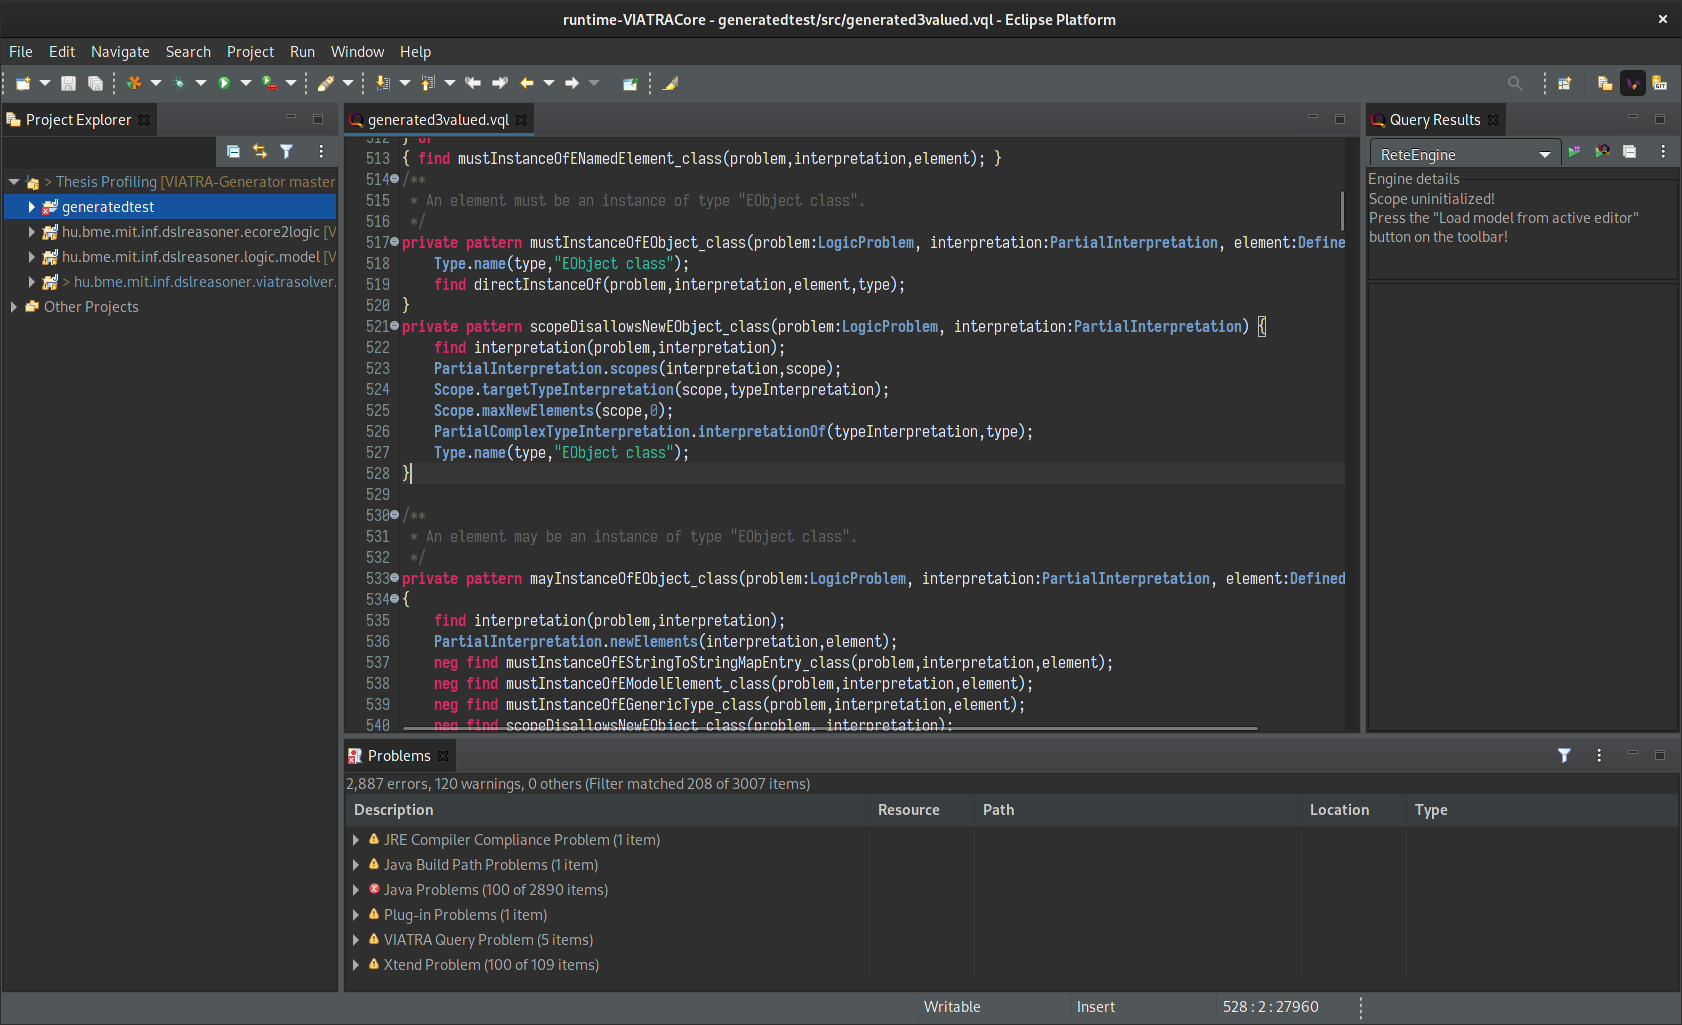
\includegraphics[width=150mm, keepaspectratio]{figures/eclipse-viatra.png}
\caption{The VIATRA Transformation Development perspective in Eclipse}
\label{fig:eclipse-viatra}
\end{figure}

\section{VIATRA Query Language (VQL)}
\subsection{Pattern matching on models}
An effective way of validating models is declaring patterns indicating incorrect
models. For example, if our model represents a family tree, we may look for
cycles.

In VIATRA Query, we can write such patterns that are matched on a loaded model.
Defining patterns is done via a powerful domain-specific language (DSL) called
the VIATRA Query Language (VQL). The VIATRA Query Eclipse plugins provide an
editor with proper syntax highlighting and code completion to make writing
patterns easier.

\subsection{Main language elements}
VQL is a datalog dialect. As such, instead of writing functions, we write
statements, which are solved on our model. The engine will try to match the
pattern on the model, and show each match in it.

\subsubsection{Writing and re-using patterns}
Patterns begin with the \texttt{pattern} keyword, followed by the name of our
pattern, and its parameter list. The body of a pattern contains statements,
which can use existing parameters, and introduce new ones.

\begin{lstlisting}[frame=single]
pattern grandparentOf(grandchild : Person, grandparent : Person) {
    Person.parent(grandchild, parent);
    Person.parent(parent, grandparent);
}
\end{lstlisting}

In this pattern, we declare a grandparent of a person, as a parent of one of its
parents. The \texttt{grandchild} and \texttt{grandparent} parameters are
explicitly given, while the \texttt{parent} parameter is introduced by the first
\texttt{Person.parent} statement. This simple pattern will match each
grandparent-grandchild relation in our model.

%% TODO:
%% Aki nem érti, hogy működik a VQL, az ebből a bekezdésből sem fogja megérteni.
%% Kell utána még egy részletesebb példa: minimum szöveggel, de akár ábrával
%% megadsz egy példánymodellt néhány Person objektummal, és bemutatod, hogy a
%% mintának a következő N darab illeszkedése lesz, ahol minden illeszkedés egy
%% grandchild-grandparent páros.
%% Ez már elvisz annyit, hogy a diszjunkció és kompozícióról szóló rész lehet új
%% subsub...section (Pattern disjunction and composition)

Patterns can have multiple declarations, and match other patterns by using the
\texttt{find} keyword. If we separately track mothers and fathers instead of
just parents, our patterns may look like the following.

\begin{lstlisting}[frame=single]
pattern parentOf(child : Person, parent : Person) {
    Person.mother(child, parent);
} or {
    Person.father(child, parent);
}

pattern grandparentOf(grandchild : Person, grandparent : Person) {
    find parentOf(grandchild, parent);
    find parentOf(parent, grandparent);
}
\end{lstlisting}

\pagebreak

\subsubsection{Pattern aggregation}
Another language feature frequently used is aggregation. You can use
aggregators for numeric results like \textbf{count}, \textbf{max}, \textbf{min},
and \textbf{sum}. This snippet counts the amount of grandparents a person has.

Any parameter with a single underscore denotes it as a known unused parameter.
In this example, we don't use the \texttt{Person} entities of the grandparents
for anything other than counting them.

\begin{lstlisting}[frame=single]
pattern grandparentAmount(child : Person, amount) {
    amount == count find grandparentOf(child, _);
}
\end{lstlisting}

%% TODO
%% Itt be kéne mutatni a check() és eval() elemeket is egy szakaszban,
%% és mondani, hogy azok a VQL-ben XBase alapúak

\subsection{Formulating constraints}
One can also provide model validation, by writing \textbf{constraint patterns}.
This can be done by annotating our validation pattern.

\begin{lstlisting}[frame=single]
@Constraint(targetEditorId = "org.dfintha.familytree",
            severity = "error",
            message = "Person is both a parent and grandparent of someone.",
            key = {"parent"})
pattern bothParentAndGrandparent(person : Person, parent : Person) {
    find parentOf(person, parent);
    find grandparentOf(person, parent);
}
\end{lstlisting}

\section{The Xtext language framework}
%% TODO
%% Ez is 2-es szakasz, azon belül viszont a VQL-re vonatkozó részletesebb
%% ismertető elé

VQL was implemented using the Xtext framework. This framework is an effective
tool for developing programming and domain-based languages.

For the languages implemented using it, the Xtext framework provides the
following services\cite{xtext}.

\begin{itemize}
    \item{language parser}
    \item{linker}
    \item{editing support in editors supporting the Language Server Protocol}
    \item{
        customizable language services, which one can build their concrete
        implementation on
        \begin{itemize}
            \item{scoping}
            \item{validation}
            \item{code generation}
            \item{outline support}
        \end{itemize}
    }
\end{itemize}

It should also be noted, that some internal parts of VQL infrastructure were
implemented using the Xtend language, which is also part of the Xtext project,
implemented in Xtext itself. Xtend is a Java dialect, with some modern language
elements, such as macros, lambdas, and operator overloading\cite{xtend}.

\section{Work environment}

%% TODO
%% ez nagyon későre való, nem is a 2-es fejezetbe

\subsection{Eclipse Platform for VIATRA development}
VIATRA, as an Eclipse plugin is developed in Eclipse itself. As such, I needed
an Eclipse environment to develop it. Normally, this should be a straightforward
process, utilizing the Eclipse Oomph installer, but at the time I did my
research the installer didn't work as expected, so I had to install the required
plugins, and add the VIATRA source code to my environment manually.

The detailed steps on how to do this is is written down on the VIATRA project
website\cite{ujhelyi_harmath_david_nagy_hegedus_2019}.

During my work, instead of installing the whole VIATRA framework, I've only
used the relevant components of VIATRA Query their dependencies, avoiding any
unrelated functionality.

\subsection{YourKit Java Profiler}
Since the main issue we have to investigate is a slowdown, I had to use a
profiler software to examine various aspects of software execution, like how
much CPU time did we spend in functions, and how many times functions were
called. Measured data is then compiled into a snapshot, on which one can perform
further analysis.

YourKit Java Profiler has three modes of profiling.
\begin{itemize}
    \item{\textbf{sampling}: measures the time spent in each function}
    \item{\textbf{call count}: measures the amount of times individual functions were called}
    \item{\textbf{tracing}: measures both time spent in functions and call counts}
\end{itemize}

\begin{table}[ht]
    \footnotesize
    \centering
    \begin{tabular}{ l l l }
        \toprule
        Mode & Measures Taken & Overhead \\
        \midrule
        Sampling & Time spent in individual functions & Moderate \\
        Call Count & Times individual functions were called & Low \\
        Tracing & Both time spent and call counts of functions & High \\
        \bottomrule
    \end{tabular}
    \caption{Profiling modes of YourKit Java Profiler}
    \label{tab:profiler-modes}
\end{table}

When using the tracing mode, we also have to opportunity to turn
\textbf{adaptive tracing} on, which ignores measuring trivially fast functions,
reducing the potential overhead it might cause.

\begin{figure}[ht]
\centering
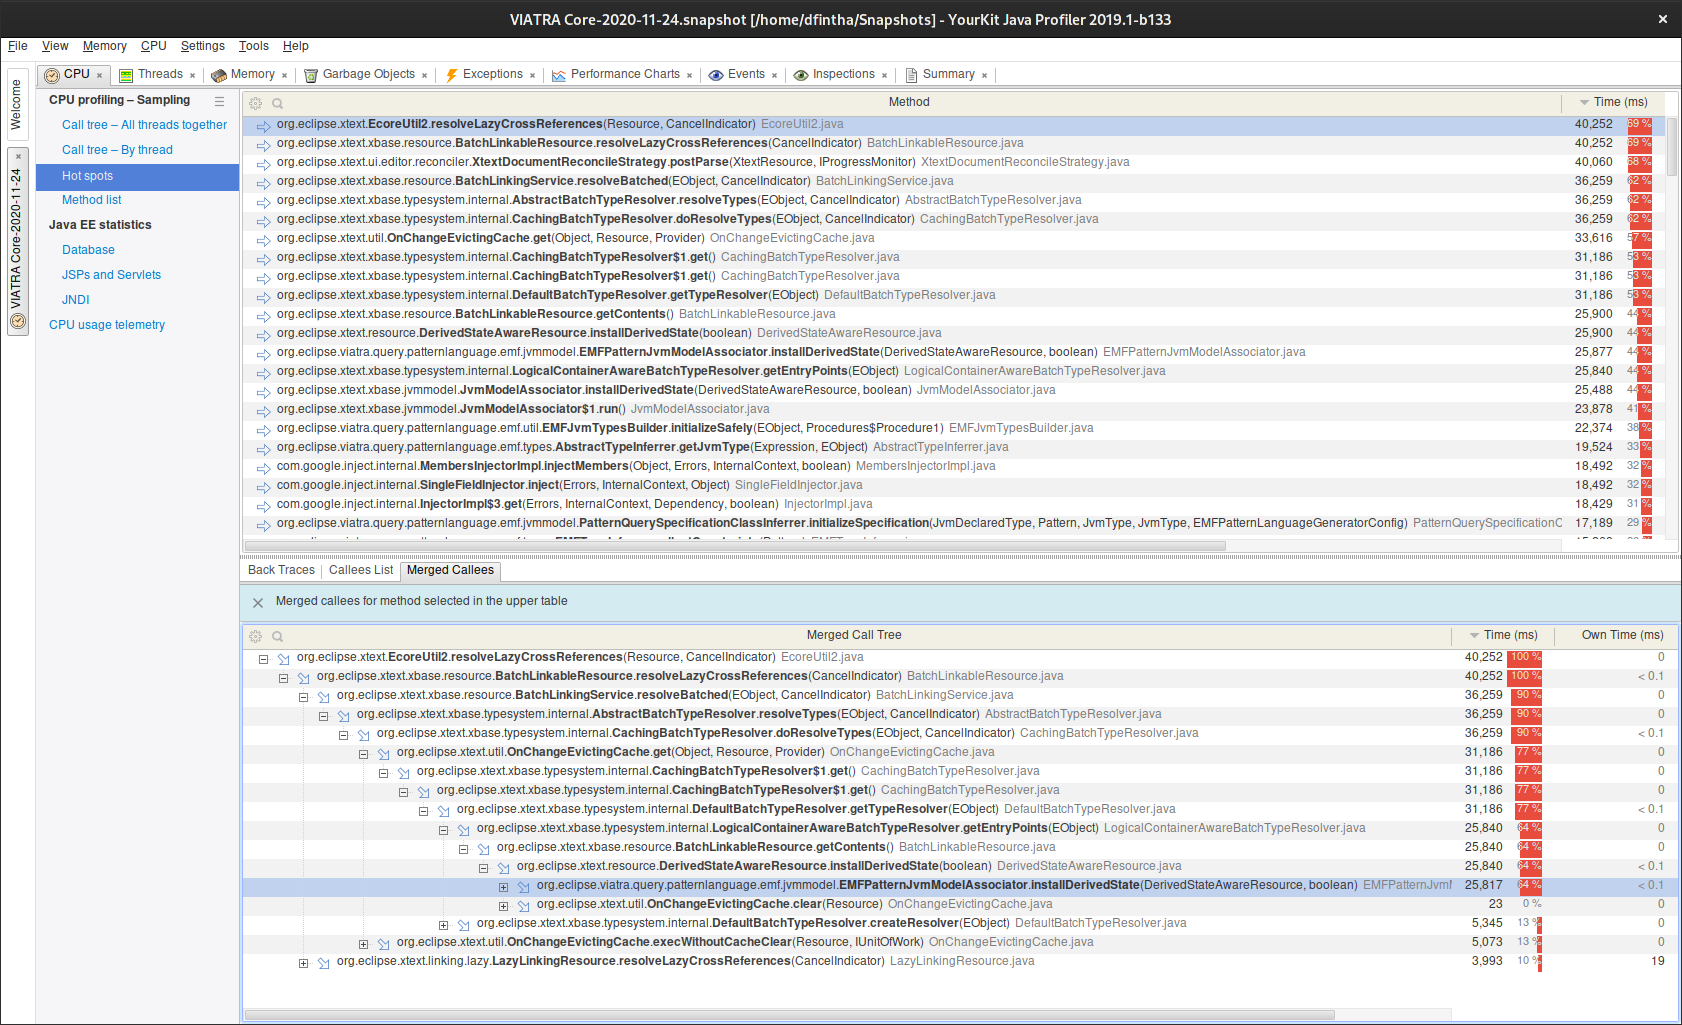
\includegraphics[width=150mm, keepaspectratio]{figures/yourkit-profiler.png}
\caption{YourKit Java Profiler in action}
\label{fig:yourkit-profiler}
\end{figure}

\pagebreak

The profiler lets us see the call tree of the profiled software or a list of its
called functions ordered by the time spent in them. It also has a ``hot spots''
mode, which highlights the costliest functions. For each function, we can also
check their backtraces, their callees, and a merged callee list, showing
in-depth information about its callees.

The above figure shows such a merged callee list of a function highlighted in
the ``hot spots'' mode.

\chapter{Finding the cause of the editor slowdown}

\section{Creating a test candidate}
To begin my work, I had to create a test project with a query, which
consistently struggles with such performance issues. The VIATRA-Generator
project\cite{github-viatra-generator} did contain a generated query file, which
had more than enough issues to slow down the workflow.

After having a proper candidate, I had to create a VIATRA
project\cite{github-viatra-vql-slowdown-example} around it, and
remove duplicated pattern code, which existed because of the generated nature
of this query. The finished query did not contain any errors, but caused massive
slowdowns -- it was perfect for my cause.

Before measuring anything with a profiler, I've conducted some manual testing,
which consisted of smaller editing sessions.

\section{Profiling the query language editor}
\subsection{Declaring a profiling workflow}
First of all, I had to create a profiling workflow, which describes the steps
taken to profile the software. Following a fixed workflow ensures that snapshots
will not contain unrelated parts of the software execution, and that snapshots
will represent the same steps taken.

\begin{enumerate}
    \item{Start VIATRA in profiling mode, but without starting profiling itself.}
    \item{Wait for Eclipse to start and finish initial tasks.}
    \item{Open the query file, and wait for it to completely load, and highlight syntax.}
    \item{
        Navigate to a certain pattern, which we will manually duplicate
        (\texttt{mustInstanceOfEClassifier\_class}).
    }
    \item{\textbf{Start profiling in the profiler software.}}
    \item{
        Manually type in the pattern again, with a different name
        (\texttt{mustInstanceTest}).
    }
    \item{Wait for the Xtext validation process to finish.}
    \item{\textbf{Stop profiling in the profiler software, and save a snapshot.}}
    \item{Quit Eclipse, discarding any changes we made in the file.}
\end{enumerate}

\subsection{Profiling with default settings}
Having a sound profiling plan, I started profiling the software. During my
first profiling session, I did notice the hangups, when I edited the query. This
session provided me with the following suspicious function trail. Each row of
one or more functions in this table was called by the one before it. Rows with
bold font are representing functions inside the VIATRA code base.

We spent most of the time in the
\texttt{XtextDocumentReconcileStrategy.postParse} function. The table below
gives detailed information about which functions called by \texttt{postParse}
were the most costly.

\begin{table}[ht]
    \footnotesize
    \centering
    \begin{tabular}{ l c }
        \toprule
        Function & Time (\%) \\
        \midrule
        XtextDocumentReconcileStrategy.postParse & 100\% \\
        EcoreUtil2.resolveLazyCrossReferences & 99\% \\
        BatchLinkableResource.resolveLazyCrossReferences & 99\% \\
        BatchLinkingService.resolveBatched & 97\% \\
        AbstractBatchTypeResolver.resolveTypes & 97\% \\
        CachingBatchTypeResolver.doResolveTypes & 97\% \\
        OnChangeEvictingCache.get & 95\% \\
        CachingBatchTypeResolver\$1.get & 95\% \\
        CachingBatchTypeResolver\$1.get & 95\% \\
        DefaultBatchTypeResolver.getTypeResolver & 95\% \\
        LogicalContainerAwareBatchTypeResolver.getEntryPoints & 92\% \\
        BatchLinkableResource.getContents & 92\% \\
        DerivedStateAwareResource.installDerivedState & 92\% \\
        \textbf{EMFPatternJvmModelAssociator.installDerivedState} & 92\% \\
        JvmModelAssociator.installDerivedState & 92\% \\
        JvmModelAssociator\$1.run & 91\% \\
        \textbf{EMFPatternLanguageJvmModelInferrer lambdas} & 78\% \\
        \bottomrule
    \end{tabular}
    \caption{Merged callee run times in postParse with default settings}
    \label{tab:postparse-default}
\end{table}

The EMFPatternLanguageJvmModelInferrer class has multiple lambdas, but the top
three with most time spent in them are all calling the
\texttt{AbstractTypeInferrer.getJvmType} method, which is responsible for their
long run time.

\subsection{Profiling without automatic update of target platform metamodels}
%% TODO
%% a "target platform" és a "metamodel" kiefejezés is itt hangzik el először
%% automatic update: be kell mutatni korábban a kapcsoló meglétét, motivációját,
%% működési elvét, hátrányát, és itt igazolni, hogy tényleg gyorsít

After turning off this automatic update feature, we can have more concise
profiling results. Repeating the same process yielded the following, similar
results. Now the \texttt{XtextDocumentReconcileStrategy.postParse} function only
took 67\% of the total run time.

\begin{table}[ht]
    \footnotesize
    \centering
    \begin{tabular}{ l c }
        \toprule
        Function & Time (\%) \\
        \midrule
        XtextDocumentReconcileStrategy.postParse & 100\% \\
        EcoreUtil2.resolveLazyCrossReferences & 96\% \\
        BatchLinkableResource.resolveLazyCrossReferences & 96\% \\
        BatchLinkingService.resolveBatched & 87\% \\
        AbstractBatchTypeResolver.resolveTypes & 87\% \\
        CachingBatchTypeResolver.doResolveTypes & 87\% \\
        OnChangeEvictingCache.get & 75\% \\
        CachingBatchTypeResolver\$1.get & 75\% \\
        CachingBatchTypeResolver\$1.get & 75\% \\
        DefaultBatchTypeResolver.getTypeResolver & 75\% \\
        LogicalContainerAwareBatchTypeResolver.getEntryPoints & 62\% \\
        BatchLinkableResource.getContents & 62\% \\
        DerivedStateAwareResource.installDerivedState & 62\% \\
        \textbf{EMFPatternJvmModelAssociator.installDerivedState} & 62\% \\
        JvmModelAssociator.installDerivedState & 61\% \\
        JvmModelAssociator\$1.run & 57\% \\
        \textbf{EMFPatternLanguageJvmModelInferrer lambdas} & 52\% \\
        \bottomrule
    \end{tabular}
    \caption{Merged callee run times in postParse without automatic update}
    \label{tab:postparse-no-auto-update}
\end{table}

In conclusion, metamodel updates are very costly, and even though turning
automatic updates off does save some time, these updates still happen
frequently and should be optimized. My next step was to understand the code
responsible for type inference, and look for opportunities to optimize it.

\subsection{The Xtext validation process}
%% TODO
%% Ez háttérismeret

To validate our query, the Xtext framework parses the query written in VQL
(partially utilizing VIATRA's code), creates a document object model (DOM) of
it, and finally, runs checks on said model. The process of building this DOM is
calling the \texttt{IDerivedStateComputer.installDerivedState} function in the
Xtext framework, which is responsible for producing the current state of our
query.

\begin{figure}[ht]
\centering
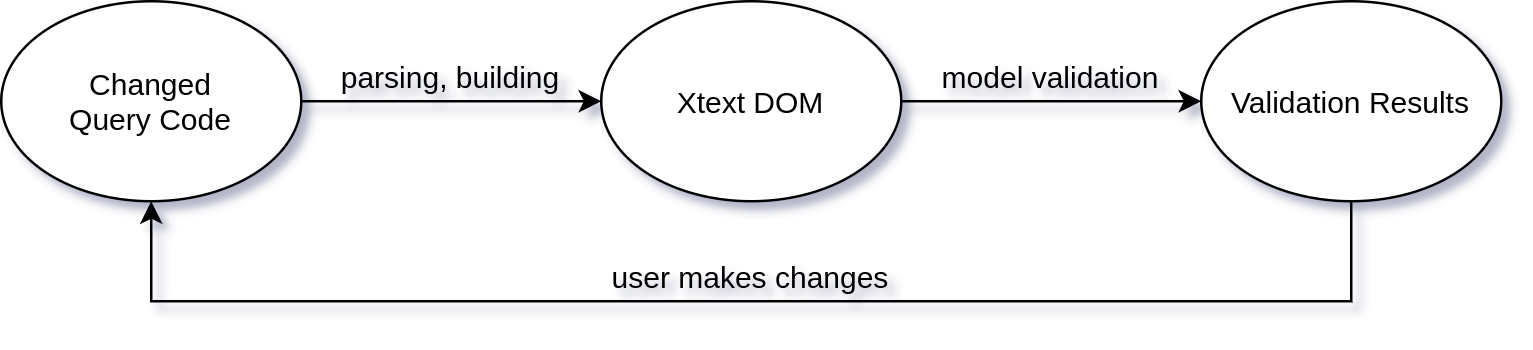
\includegraphics[width=150mm, keepaspectratio]{figures/xtext-validation-process.png}
\caption{The Xtext validation process}
\label{fig:xtext-validation-process}
\end{figure}

The slowest part of this process is building the DOM from the parsed query code.
During model building, the types of variables must be interpreted, and while
most of these variables have a \textbf{declared type}, some of them do not, and
VIATRA Query has to \textbf{infer their types} based on the context they reside
in.

%% TODO
%% Példa inferred és declared type-ra

My choice of optimization is implementing a cache for the
\texttt{AbstractTypeInferrer}, to avoid repeated inferences of the same type.
Since it takes a large part of the run time (33\% without automatic update,
and 75\% with it), the speedup should be significant.

\chapter{Optimizing query metamodel generation}
\section{Implementing a type inferrer cache}
\subsection{Inspecting the original functionality}
During the type inference process, \texttt{getJvmType} is called numerous times,
resulting in a massive amount of processing time spent there. Let us see, how
this function works.

\begin{lstlisting}[language=java]
// ...

/**
 * @since 1.3
 */
@Override
public IInputKey getType(Expression ex) {
    final IInputKey declaredType = getDeclaredType(ex);
    if (declaredType != null) {
        return declaredType;
    } else {
        return getInferredType(ex);
    }
}

//...

/**
 * @since 1.3
 */
@Override
public JvmTypeReference getJvmType(Expression ex, EObject context) {
    return typeSystem.toJvmTypeReference(getType(ex), context);
}

// ...
\end{lstlisting}

The profiling session showed us that we spend most of the time in the
\texttt{getType} function, and inside that, the \texttt{getInferredType}
function, which actually does a costly type calculation, and does so repeatedly.
This looks like a good candidate for some caching mechanism.

\subsection{Caching computed results}
My first approach was adding a cache to the \texttt{AbstractTypeInferrer} class,
storing the types (\texttt{IInputKey}) of \texttt{Expression} objects. I thought
this cache would be invalidated at the start of each validation process. As
such.

The following changes were made to the \texttt{AbstractTypeInferrer} class.

\begin{lstlisting}[language=java]
// ...

private HashMap<Expression, IInputKey> typeCache;

// ...

/**
 * @since 1.3
 */
@Override
public IInputKey getType(Expression ex) {
    if (typeCache == null)
        typeCache = new HashMap<>();

    return typeCache.computeIfAbsent(ex, expression -> {
        final IInputKey declaredType = getDeclaredType(expression);
        if (declaredType != null)
             return declaredType;
        return getInferredType(expression);
    });
}

// ...
\end{lstlisting}

\subsection{Clearing the cache}
Since the type inferrer, which caches the types is thrown away when then
\texttt{OnChangeEvictingCache} is cleared, there is no need to manually clear
its type cache.

\subsection{Comparing the optimized state with the original one}
After making these changes, I did another profiling session, with the same
workflow described above. Seemingly my first solution did not fully accomplish
my goal, the run time of the validation process remained close to the same. The
\texttt{XtextDocumentReconcileStrategy.postParse} function still ate up 64\% of
the runtime (compared to the original 67\%), but the type inference code became
slightly faster.

\begin{table}[ht]
    \footnotesize
    \centering
    \begin{tabular}{ l c c }
        \toprule
        Function & Time (\%), Original & Time (\%), Changed \\
        \midrule
        XtextDocumentReconcileStrategy.postParse & 100\% & 100\% \\
        EcoreUtil2.resolveLazyCrossReferences & 99\% & 95\% \\
        BatchLinkableResource.resolveLazyCrossReferences & 99\% & 95\% \\
        BatchLinkingService.resolveBatched & 97\% & 84\% \\
        AbstractBatchTypeResolver.resolveTypes & 97\% & 84\% \\
        CachingBatchTypeResolver.doResolveTypes & 97\% & 84\% \\
        OnChangeEvictingCache.get & 95\% & 70\% \\
        CachingBatchTypeResolver\$1.get & 95\% & 70\% \\
        CachingBatchTypeResolver\$1.get & 95\% & 70\% \\
        DefaultBatchTypeResolver.getTypeResolver & 95\% & 70\% \\
        LogicalContainerAwareBatchTypeResolver.getEntryPoints & 92\% & 58\% \\
        BatchLinkableResource.getContents & 92\% & 58\% \\
        DerivedStateAwareResource.installDerivedState & 92\% & 58\% \\
        \textbf{EMFPatternJvmModelAssociator.installDerivedState} & 92\% & 58\% \\
        JvmModelAssociator.installDerivedState & 92\% & 57\% \\
        JvmModelAssociator\$1.run & 91\% & 54\% \\
        \textbf{EMFPatternLanguageJvmModelInferrer lambdas} & 52\% & 48\% \\
        \bottomrule
    \end{tabular}
    \caption{Comparison of run time with the unmodified code and my first solution}
    \label{tab:first-solution-comparison}
\end{table}

The suspicious part was the ratio of the time spent in functions called by the
\texttt{getType} function. The purpose of my cache was minimizing calls to the
\texttt{getInferredType} function, which took the most time. However, the amount
of time spent in the \texttt{getInferredType} function was roughly the same (
77\% and 76\%, respectively).

My first suspicion was that \texttt{Expression} objects are never the ``same'',
so two \texttt{Expression}s with the same content evalute to two different
hashes, and my cache always misses.

\pagebreak

To make sure, I did another profiling, now in trace mode. Trace mode means
counting function calls along with time spent with them, which may seem like the
best way to profile software, but this mode comes with a major slowdown, making
it harder to perform the profiling workflow.

\begin{table}[ht]
    \footnotesize
    \centering
    \begin{tabular}{ l c c c }
        \toprule
        Function & Time (\%) & Count & Count (\%) \\
        \midrule
        (total calls to getType) & 100\% & 13346 & 100\% \\
        EMFTypeInferrer.getInferredType & 97\% & 121 & 0.009\% \\
        EMFTypeInferrer.getDeclaredType & 3\% & 2245 & 0.168\% \\
        \bottomrule
    \end{tabular}
    \caption{Time and call count of callees of \texttt{getType} with my first solution}
    \label{tab:first-solution-call-counts}
\end{table}

In previous profiling sessions of the original code, I've used the sampling
mode. To compare the results, I also had to perform a tracing profiling session
using the original source. The results can be seen below.

\begin{table}[ht]
    \footnotesize
    \centering
    \begin{tabular}{ l c c c }
        \toprule
        Function & Time (\%) & Count & Count (\%) \\
        \midrule
        (total calls to getType) & 100\% & 24733 & 100\% \\
        EMFTypeInferrer.getInferredType & 97\% & 276 & 0.01\% \\
        EMFTypeInferrer.getDeclaredType & 3\% & 24731 & 99.99\% \\
        \bottomrule
    \end{tabular}
    \caption{Time and call count of callees of \texttt{getType} with the original source}
    \label{tab:first-solution-call-counts}
\end{table}

Please note, that during the measurement of the original source, the minimal
difference between the amount of \texttt{getType} and \texttt{getDeclaredType}
call counts may be attributed to the termination of the profiling session, while
an Xtext validation process was still in progress.

The results of these trace mode profilings have proven my suspicion partially
false. The most part of the \texttt{getType} function was still spent in
\texttt{getInferredType}, but my cache helped avoid some repeated calculations.

\subsection{Conclusion}
If we look at the previous implementation of \texttt{getType}, we can see that
\texttt{getDeclaredType} was called the same amount of times as
\texttt{getType} itself, but if it failed, we fell back to
\texttt{getInferredType} After adding the type cache, the call count of the two
functions added dropped to only 17.7\% of the total call count. This means that
\textbf{82.3\% of times the cache did not miss}.

\pagebreak

\section{Fine-grained type caching}
Caching the calculated types did accomplish a minor speedup, but the editor
still hangs up during Xtext validation.

The Xtext framework caches information during file processing in a cache, but as
soon as the file is changed, the cache is evicted, and this information is lost.
My additional type cache helped keep some values cached \textbf{during this
processing, avoiding re-calculation of the same type in one process}, but some
of the values still need to be recalculated.

To further optimize the process, these calculated types for expressions could
be kept in a cache that persists between changed states, as long as the meaning
of those expression remain the same. This could result in an additional
significant speedup.

Looking for such a cache mechanism, I studied the Xtext framework documentation
for a cache other than \texttt{OnChangeEvictingCache}, but on developer forums,
it was explicitly stated to be nonexistent\cite{xtext-fine-grained-caching}. As
such, I had to look for another solutions.

\section{Improving type inference performance}
%% TODO
%% TypeInformation.(getType|getAllTypes|getMinimizedTypes)
%% EMFTypeInferrer.collectConstraints
%%   PatternLanguageHelper.getReferencedPatternsTransitive
TODO

\chapter{Publishing my work}
\section{Documenting the changes}
It is just natural, that we would document the changes we've made to the users,
even if it's not a functional change. The VIATRA documentation is written in
asciidoc format, and each release has its own changelog.

These documentation files are stored in the
\texttt{org.eclipse.viatra.documentation.help} package. Documenting my work was
as simple as adding a new line to the ``New and Noteworthy'' section of the
release documentation for the upcoming VIATRA version (2.5).

\section{Opening a bug tracker ticket}
The Eclipse Foundation uses Bugzilla as its bug tracker. Each known bug has a
ticket assigned, and this ticket has a unique identifier. Tickets contain
a detailed description of the issue, and some other metadata, such as product,
version, importance, and target milestone. These tickets then can be assigned to
developers.

For this thesis work, a new Bugzilla ticket was introduced:
Bug 569178 -- Improve language tooling performance.

\begin{figure}[ht]
\centering
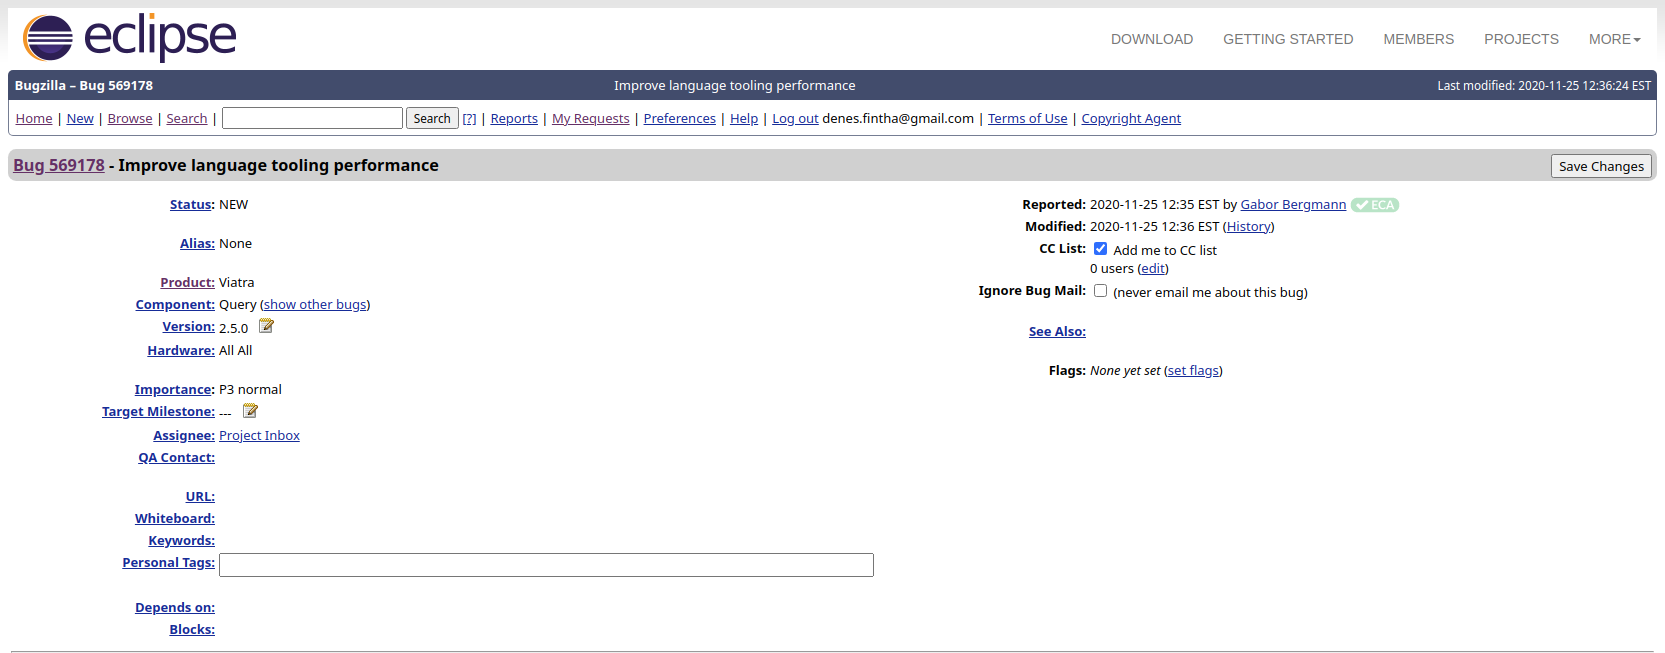
\includegraphics[width=150mm, keepaspectratio]{figures/bugzilla.png}
\caption{Eclipse Foundation's Bugzilla bug tracker}
\label{fig:bugzilla}
\end{figure}

\pagebreak

\section{Keeping the changes in version control}
VIATRA source code is stored in a Git repository, hosted by the Eclipse
foundation. To obtain the source code, developers have to \textbf{clone} the
repository, and work can be done on their own \textbf{branches}. Git has a
command-line tool, but Eclipse can also manage version control by using the
Git perspective.

\begin{figure}[ht]
\centering
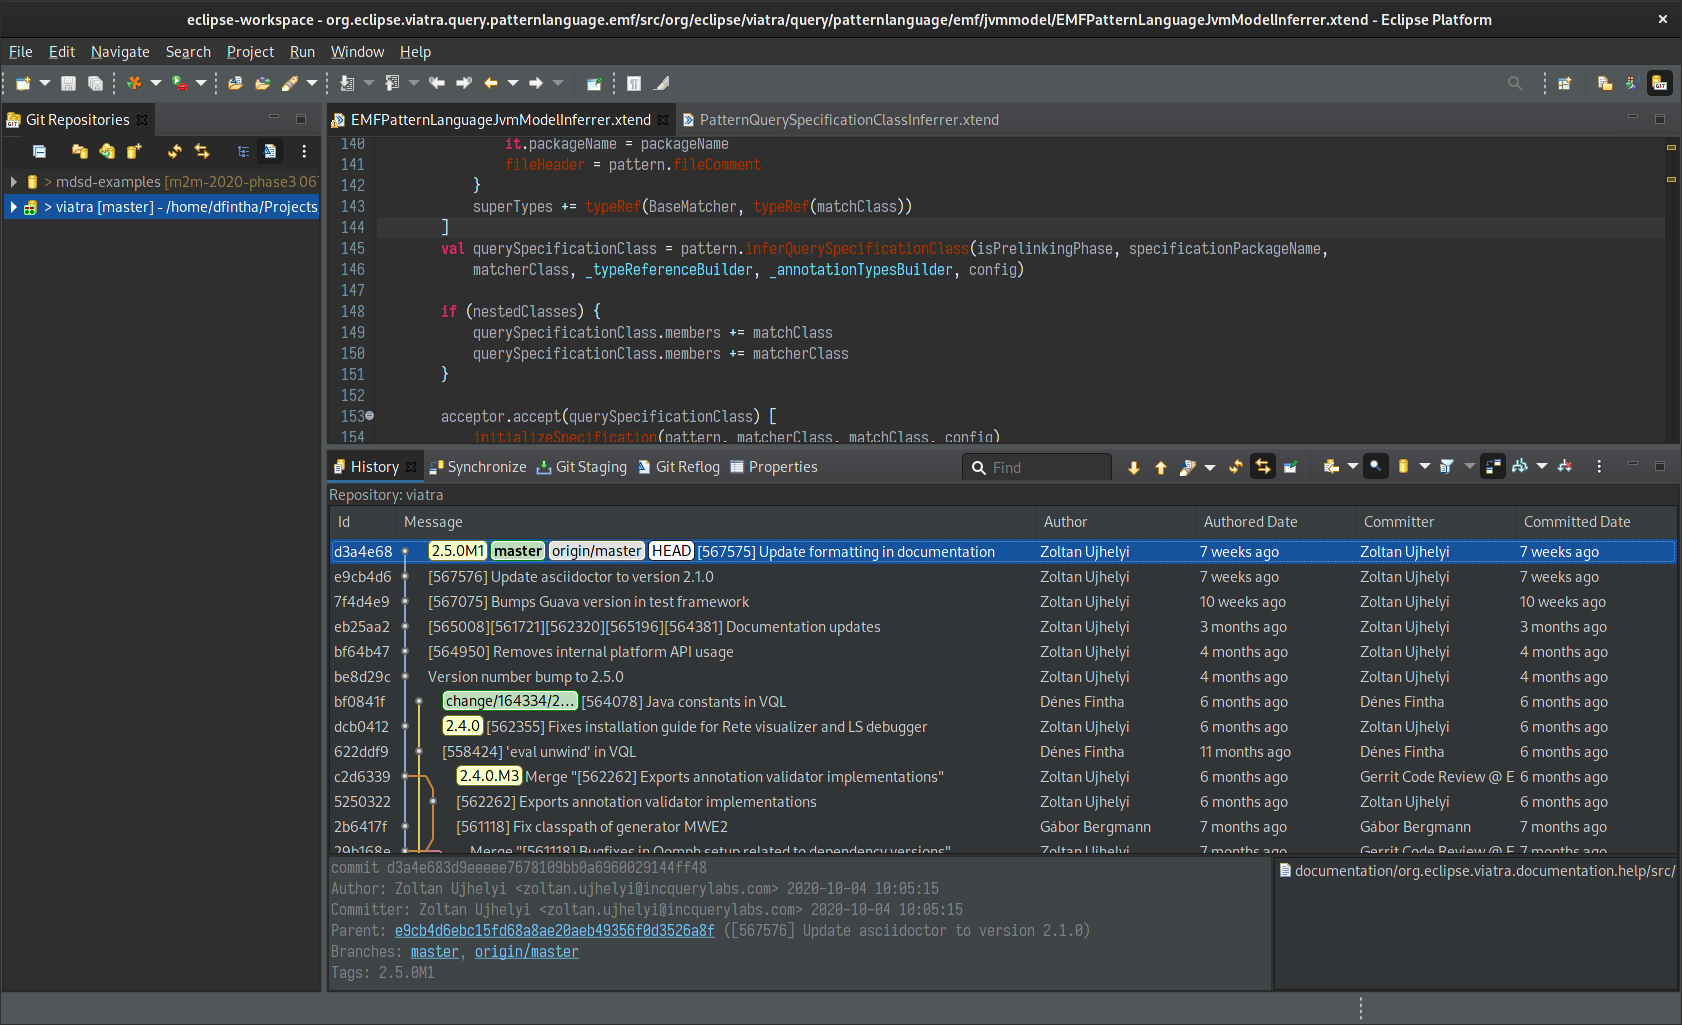
\includegraphics[width=150mm, keepaspectratio]{figures/eclipse-git.png}
\caption{The Git perspective in Eclipse}
\label{fig:eclipse-git}
\end{figure}

Changes on the source code are contained in \textbf{commits}, and in Eclipse
development each bug fixing commit correlates with a Bugzilla ticket, and
should include the bug identifier and title in its commit message, along with
a short description, sign-off information that proves the changes in the commit
were made by me, and a change ID for the code review tool.

\begin{lstlisting}
[569178] Improve language tooling performance

This commit introduces a caching mechanism for the AbstractTypeInferrer
class, allowing it to cache inferred types and avoiding repeatedly
calculating the types of expressions.

Change-Id: I0000000000000000000000000000000000000000
Signed-off-by: Dénes Fintha <denes.fintha@gmail.com>
\end{lstlisting}

\pagebreak

\section{Code review}
Before any code could be integrated to the mainstream VIATRA source, peer review
must be conducted. The Eclipse Foundation uses Gerrit to do so, which is a
web-based code review tool.

Gerrit supports multiple versions of the same commit, identified via a
\texttt{Change-Id}, which is denoted in the commit message.

In Gerrit, developers can see other developers' work, and comment and rate their
commits. Each organization can have their own rules about peer review, i.e. two
other developers must accept a commit before its integration.

\begin{figure}[ht]
\centering
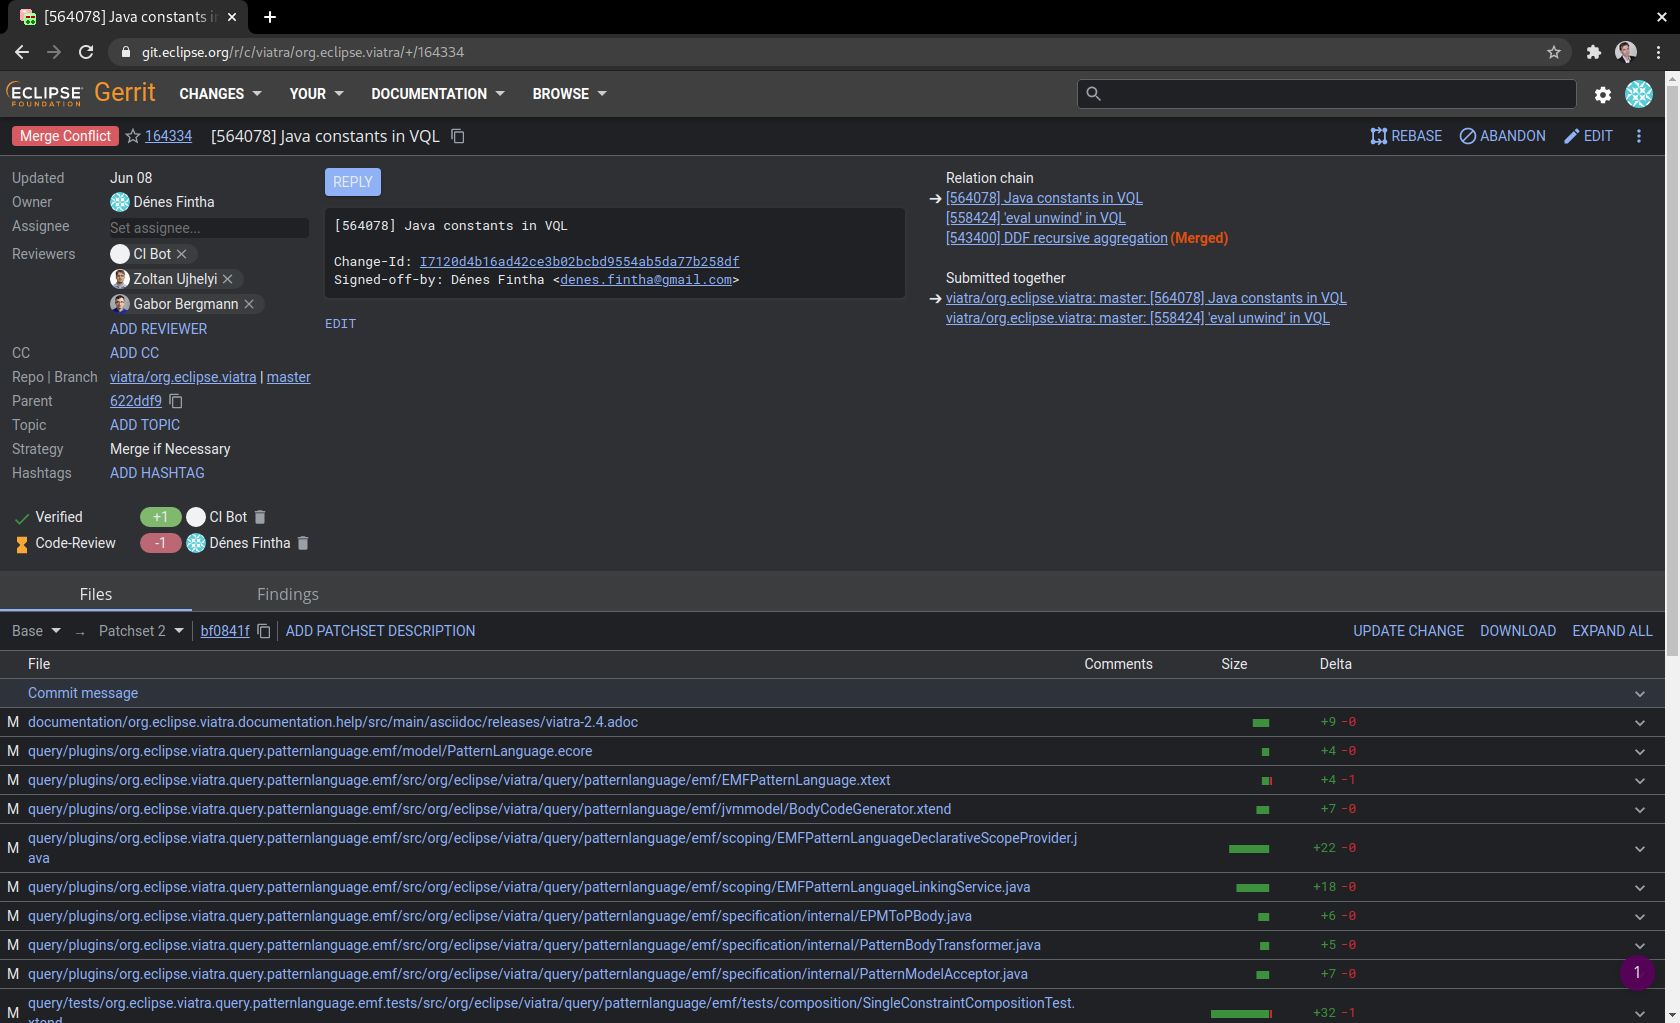
\includegraphics[width=150mm, keepaspectratio]{figures/gerrit.png}
\caption{The Gerrit Code Review tool}
\label{fig:gerrit}
\end{figure}

\section{Integrating changes to the next VIATRA version}
%% TODO
%% Integration process
TODO

\chapter{Summary}
This thesis work was centered around investigating a large existing project, and
finding and fixing performance issues. Although most of the issues originated
from an external framework, I did manage to achieve a small performance
increase, which I consider a success.

\section{Improvement opportunities}
%% TODO
TODO

\subsection{Fine-grained caching in the Xtext framework}
%% TODO
TODO

% ---------------------------------------------------------------------------- %

\listoffigures\addcontentsline{toc}{chapter}{\listfigurename}
\listoftables\addcontentsline{toc}{chapter}{\listtablename}
\addcontentsline{toc}{chapter}{\bibname}
\bibliography{bib/mybib}
\label{page:last}

\end{document}
